\section{Own Experiments}
\label{own-experiments}
To predict the correct number of a given verb,
the language model should be able to
1. identify the noun that is the head of the subject for the verb
2. establish the number of the noun (non-trivial since no knowledge of -s postfix for plurals)
3. establish the number of the given verb forms (also non-trivial).

In the first sub section we investigate if our model is able to
do this for simple cases with only a single noun in the prefix.
%
In the second sub section we investigate if our model can handle
more complex cases with two nouns in the prefix,
and what information it then uses to identify the head of the subject.

%TODO: describe model (or in previous section)

\subsection{Noun-Verb Agreement in Simple Cases}

In this section we further investigate the ability of the model to
establish number agreement for nouns and verbs in the simplest case
following the pattern: ``The <noun> <verb>''. Notice that
the determiner ``The'' clearly indicates the position of the subject.
From this we hope to get insights whether or not the model is sensitive to noun-verb agreement, i.e. if the model tends to predict plural verbs for plural nouns and singular verbs for singular nouns.


Using the 40 most frequent nouns and verbs that we already used earlier in the replication section, we generated 80 x 40 sentences. To evaluate how the language model is going to perform on these sentences we tested, for each noun-verb combination, how likely the model is going to predict the singular and the plural verb respectively.

As a result of this evaluation we obtained a matrix in which the entries indicate the models preference for the singular/plural verb. We calculate each value
\begin{equation}
	v = P(<VBP>)/ P(<VBP> + P(<VBZ>), 
\end{equation}
where P is the models prediction probability, <VBP> is the plural verb and <VBZ> the singular verb. In this manner the matrix provides a ratio for singularity ($v=0$) and plurality($v=1$). We call $v$ the \textit{plurality preference}. To upper part of the matrix contains all noun-verb combinations for the singular nouns, where the lower part contains the plural nouns. 

In order to get a better visual impression we sorted the columns after the sums of the columns. The rows were sorted in a similar manner, but separately in order to conserve the separation between singular (upper half) and plural (lower half) nouns. The resulting matrix is shown in Fig. \ref{fig:matrix_ratio}.

As we expected the majority of the verbs in the upper half of the matrix are predicted correctly to be singular with a high certainty. The same for the lower, plural half. Overall it can be said that the Around the horizontal axis as well as at the borders we can observe that there are specific verb/noun combinations for which the model is rather uncertain. This also matches our expectations that there are regions in the matrix where the model is not clearly in favour of the singular or plural verb. In the following we will investigate the two special cases of verbs and nouns. 

In the columns close to the left border of the matrix, we can find verbs of which the model prefers the plural verb over the singular, regardless the number of the subject. For example the verb `buy` in column 0 has a plurality preference of 0.95. In the far right columns we find the verbs of which the plural verb is preferred over the singular. The verb `say` in column 39 has a plurality preference value of 0.1625.

There are also nouns which clearly prefer one number over another. Around the middle of the matrix we can observe a few words that are clearly predicted wrong most of the times. The noun `income` with a plurality rate of 0.15 is mostly predicted singular whereas for example the words `weeks` (0.9) column 40, `months` (0,9) column 41, `years` (0,85) column 43, `days` (0,7) column 44, are predicted plural most of the times.

To investigate the impact of the frequencies in the training data on the plurality rate (and therefore on the error) further, we calculated the error rate for each noun and plotted it against the frequency of the same noun. We expected a high error rate for low frequent nouns. As the Fig. \ref{fig:noun_freq_error} shows there is no clear evidence that a low frequency of singular or plural nouns in the training data leads to mistakes of the model. Figure \ref{fig:noun_freq_error} shows that there are singular as well as plural nouns with a low count that are predicted correctly most of the times (error rate < 0.2). 

The previous experiment neglects the fact that even though a word is frequent in the corpus it could never be the subject in the training sentence. We investigated whether the nouns that we encountered before as being predicted wrong most of the times, namely: `weeks`,`months`, `years` and `days` are in fact rarely the subject in the training data. This suggests that the model is not indeed not able to establish the number agreement for nouns and verbs in a more general but rather in a statistical way. Figure \ref{fig:lin_reg} supports this assumption. It shows the plurality rate plotted against the plurality preference for each verb. We can see that with an increasing plurality rate the plurality preference increases, as expected. The line in the figure was generated by performing a linear regression through the points. 





\end{multicols}

\begin{figure}
    \centering
    \begin{subfigure}[b]{0.32\textwidth}
    \caption{}
        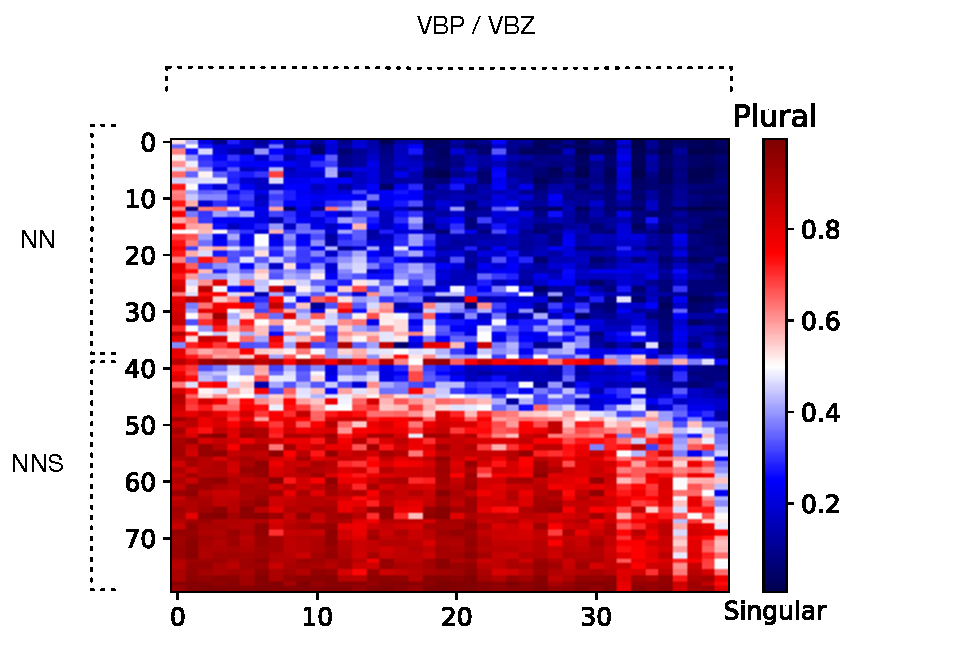
\includegraphics[width=\textwidth]{matrix_plot_ratio.pdf}
        \label{fig:matrix_ratio}
    \end{subfigure}
    ~ %add desired spacing between images, e. g. ~, \quad, \qquad, \hfill etc. 
      %(or a blank line to force the subfigure onto a new line)
    \begin{subfigure}[b]{0.32\textwidth}
    	\caption{}
        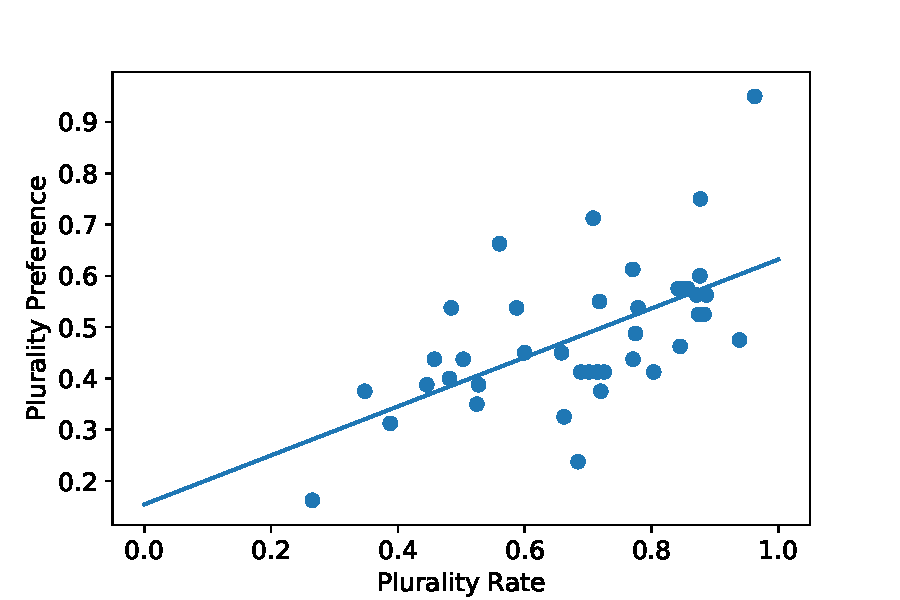
\includegraphics[width=\textwidth]{lin_reg.pdf}
        \label{{fig:matrix_ratio}}
    \end{subfigure}
        \begin{subfigure}[b]{0.32\textwidth}
    	\caption{}
        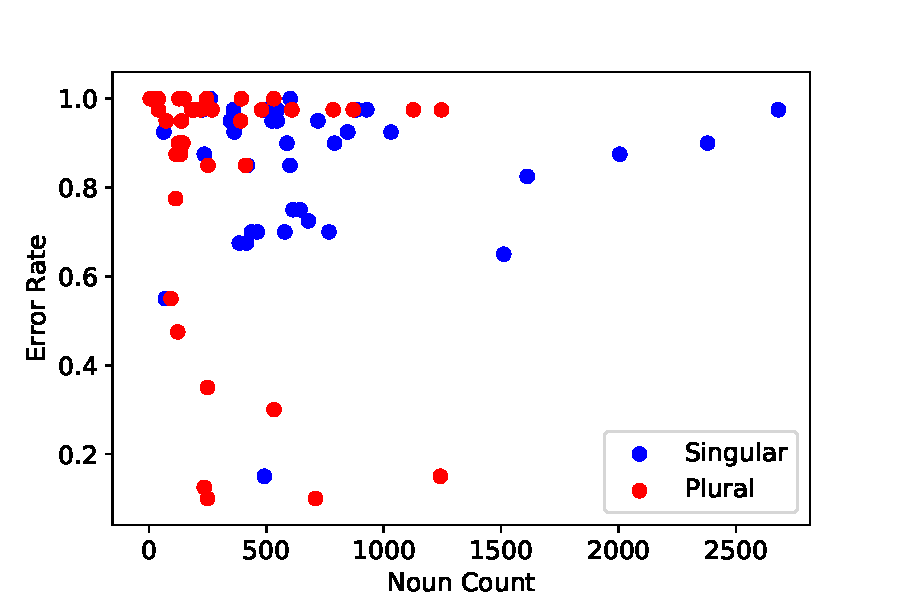
\includegraphics[width=\textwidth]{noun_freq_error_rate.pdf}
        \label{fig:noun_freq_error}
    \end{subfigure}
    \caption{\ref{fig:matrix_ratio} singularity/plurality ratio for 80 x 40 sentences (generated from the most frequent 40 nouns and verbs). The upper half contains the singular nouns (NN), the lower half contains the plural nouns(NNS). A red cell indicates a plural preference for a specific word/noun combination, whereas a blue cell indicates a singular preference. \ref{fig:matrix_ratio} plurality rate plotted against the plurality preference of the model for all nouns. The line arises from a linear regression through the points. \ref{fig:noun_freq_error} influence of the noun frequency on the error rate of the model.}
\end{figure}

\begin{multicols}{2}
\subsection{Noun-Verb Agreement in Complex Cases}

In Section \ref{replication} we analysed the performance of the model
on complex sentences, containing one or more 
nouns.
The results show that the model is very
sensitive to the most recent noun,
performing worse-than-chance with only one single attractor.
%(Figure \ref{fig:2c}). 

In this section we investigate whether
syntactic and semantic information
can still help the model 
to establish number agreement
in case of multiple nouns.
We focus on sentences with exactly two nouns
of opposite number.


\subsubsection{Syntactic Information}

%%%%% OBJECTIVE
Function words such as `that' or `of' carry 
important information about the syntactic structure of a sentence.
In this Section we investigate if the model
uses this information to establish number agreement
for complex sentences.

%%%% TEST DATA
We generated sets of sentence prefixes using 
different syntactic templates.
An example is ``The \_ of the \_''
We instantiate these templates by randomly
picking two nouns and a verb 
from a set of frequently used nouns and verbs. 
Each combination of nouns and verbs instantiates
two prefixes that differ by their plurality.
For example ``The company of the governments''
and ``The companies of the government'',
with the option to choose between the verb forms
`know' and `knows'.
Since the nouns and verbs are randomly picked,
the generated prefixes 
are typically not semantically
meaningful.

We generated 2 x 1000 sentences per template,
for a total of 11 templates.
The sentences for each template are constructed using the same
noun and verb combinations.
We defined 7 templates for which the first noun is 
the head of the subject (table \ref{tab:attractor_templates}),
while 4 templates have the second noun as the head of the subject
(table \ref{tab:lastnoun_templates}).
The templates were defined after a manual inspection
of sentences from the corpus.

%%%% EXPERIMENT:
We evaluate how the model responds to the generated test inputs.
That is, for each test prefix we let the model decide between 
the singular and plural form of the given verb. 
We measure the error rate for each template.
However, instead of showing the error rates we
show how much the language model tends to agree with the most recent noun.
This corresponds to the error rate for the templates in table \ref{tab:attractor_templates},
while it corresponds to accuracy for the templates in table \ref{tab:lastnoun_templates}.
Showing the `last noun agreement rate' makes it easier
to compare the behavior of the model for different templates.

%%%% ANALYSIS:
The results are shown in Figure \ref{fig:last_noun_rates},
using green and red colors to indicate if 
the last noun is actually the head of the subject (green)
or not (red). 
%
We see that all bars are above the 0.5 rate,
which shows that the model is most
likely to agree with the last noun,
even in cases where this is syntactically incorrect. 
%
We also see that the red bars are slightly
lower than the green bars,
0.67 compared to 0.79 on average.
This shows that the model is even more likely
to prefer the last noun if this is
also syntactically correct.
This suggests that the model has 
at least some sensitivity
to syntactic information carried by function words.
%

%
We further discuss two special cases,
namely the first red bar (T1) and 
the last green bar (T11).
T1, ``the \_ and the \_ '', is a special case because it 
actually contains two singular nouns
instead of one singular and one plural noun. 
The predicted verb should be plural because of the
conjunction word `and'.
The existence of two singular nouns 
makes it hard for the model
to pick the plural verb,
which could explain the high error rate
for T1 in Figure \ref{fig:last_noun_rates}.
%
T11 uses different templates for the singular 
(the \_ 's \_ ) and the plural (the \_' \_) possessive form.
The last green bar in Figure \ref{fig:last_noun_rates} shows the average result.
We suspect that the relatively low accuracy
in this case might be explained by the infrequent
occurrence of the plural possessive form in written text.
Indeed, a closer inspection of the numbers showed that
the singular template had an accuracy
of 0.77 (compared to 0.71 for all singular prefixes), 
while the accuracy of the plural template
was lower, namely 0.66 (compared to 0.63 overall for plural prefixes).
%

%%%% DISCUSSION / CONCLUSION:
We conclude that, although the model 
performs poorly on syntactically complex sentences it
still shows some sensitivity for syntactic 
information exposed by function words. 


\begin{Figure}
    \centering

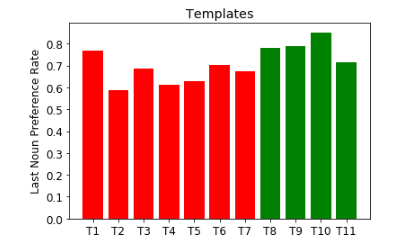
\includegraphics[scale=0.5]{screenshot-syntactic-templates} 
\captionof{figure}{Preference rates for agreement to the last noun.
The colors indicate whether this is syntactically correct (green)
or incorrect (red).
}
%TODO: save picture instead of making screenshot 
%TODO title Templates below
\label{fig:last_noun_rates}
\end{Figure}


\end{multicols}{2}



 
\begin{table}[t] 
\parbox{.45\linewidth}{
\centering
\begin{tabular}{ l l r }
  T1    & the \_ and the \_     &  0.77 \\
  T2    & the \_ in the \_      &  0.59 \\
  T3    & the \_ by the \_      &  0.69 \\
  T4    & the \_ of the \_      &  0.61 \\
  T5    & the \_ near the \_    &  0.63\\
  T6    & the \_ at the \_      &  0.70\\
  T7    & the \_ without the \_ & 0.67  \\
\end{tabular}
\caption{Templates for which the number of the verb 
is opposite to the number of the last noun} 
\label{tab:attractor_templates}
}
\hfill
\parbox{.45\linewidth}{
\centering
\begin{tabular}{ l l r }
  T8    & the \_ the \_         &  0.78\\
  T9    & the \_ that the \_    &  0.79\\
  T10   & the \_ whether the \_ &  0.85\\
  T11   & the \_ 's \_ (for plural: the \_' \_)          &  0.72 \\
\\
\\
\\
\end{tabular}
\caption{Templates for which the number of the verb 
corresonds to the number of the last noun} 
\label{tab:lastnoun_templates}
}
\end{table}

\begin{multicols}{2}


\subsubsection{Semantic Information}

We now look at semantic clues, i.e. companies
are more likely to produce than employees.
We investigate if the model is able to establish
number agreement between the verb and the semantic related noun,
ignoring the non-semantic related attractor noun.
  
1. TEST DATA:
We construct a testset (100+ sentences) consisting of pairs with singular and plural prefixes, in the following format  
``The NN of the NNS ...[VBZ/VBP]'' and
``The NNS of the NN ...[VBZ/VBP]'' 
whereby the head of the subject (the first noun)
is semantically related to the verb, while the attractor (the second noun)
is randomly picked. An example is:
``The prices of the employee ...[stabilizes/stabilize]'' and 
``The price of the employees ...[stabilizes/stabilize]''.

In addition we construct a comparison set consisting of the same prefixes
(same verb and attractor noun),
but with the difference that the first noun is also randomly picked and
therefore most likely not semantically related. Example:
``The newspapers of the employee ...[stabilizes/stabilize]'' and 
``The newspaper of the employees ...[stabilizes/stabilize]''.


EXPERIMENT:
Evaluate our model on the constructed testset and on the comparison set.
If the model scores significantly better on the testset
then it shows sensitivity to semantic clues.

%(remark: we can repeat the experiment with the nouns interchanged and check that we %score worse now,
%e.g. "The employee that the prices ... [stabilize/stabilizes]" 
%In that case syntax and semantics are inconsistent)

HOW TO FIND CO-OCCURRENCE RATIOS
We use PMI to measure associations between verbs and nouns.
%(https://en.wikipedia.org/wiki/Pointwise_mutual_information#Applications)


\begin{itemize}
\item find all nouns (NN) and verbs (VBZ) in a tagged corpus 
(sec02-21.gold.tagged).
(pick a random selection if all is too much
but make sure you are not only looking at
frequent verbs since they tend to be general like 'is/are'
instead of specific like 'stabilize')
\item  build a matrix with nouns as rows and columns as verbs
\item  fill entries with Count('noun and verb co-occur in a sentence')
i.e. loop over all sentences and add one if noun and verb exists in sentence
(or use skip grammar, but only count noun that appears before verb, see also lab4)
\item  Also keep track of the total occurrences for the Verbs and nouns
\item replace each enty by the PMI calculated from the 
co-occurrence count, the total occurences of the noun, and the occurences
of the verb
\item select for each column the entry with the highest score(s)
(you may ignore very general verbs like is/are)
\end{itemize}

Remark: can be learned from tagged data set, no need to look at training data




